\subsection{System actors}

Based on the requirements analysis, we have determined two types of actors in our system:

\begin{description}
	\item[Folder] \label{actors:folder} - A person who carries out the most important functionality in our system,
		that is - folds the origami figure following the provided interactive instruction.
		This person does not need to have any special knowledge about origami creation nor the simulation process.
	\item[Designer] \label{actors:designer} - A person who is responsible for providing folding instructions
		for other users (\textit{folders}).
		A Designer is required to have some basic knowledge about origami construction
		and interaction with the system to be able to create and upload an Instruction.
\end{description}

\newcommand{\requirement}[2]{\item #2. (#1)}
\subsection{Functional requirements}
\label{section:functional-requirements}

We provide functional requirements for the system as User Stories divided by actor type.
They have a priority assigned to them that ranges from 1 to 3. Where:

\begin{enumerate}
	\item[(3)] high priority - a feature required for the system functionality 
	\item[(2)] medium priority - a feature that is important, but not essential for the system functionality
	\item[(1)] low priority - a feature that is nice to have, but not required 
\end{enumerate}

\subsubsection{Folder user stories}
As a folder I am able to\ldots
\begin{enumerate}
	\requirement{3}{load an Instruction}
	\requirement{3}{view the 3D representation of the Instruction step}
	\requirement{3}{switch to the next step in the Instruction}
	\requirement{3}{switch to the previous step in the Instruction}
	\requirement{3}{see the Transition between two Instruction steps}
	\requirement{2}{pause the Transition at any time}
	\requirement{2}{rewind the Transition}
	\requirement{2}{forward the Transition}
	\requirement{3}{rotate the Model in 3D space}
	\requirement{3}{zoom the Model in and out in 3D space}
	\requirement{1}{see creases of the Model} 
	\requirement{2}{distinguish paper's top and bottom sides} 
	\requirement{1}{change the color of the paper side} 

	\requirement{3}{navigate between simulator and community views} 
	\requirement{3}{view Instructions uploaded by other users} 

	\requirement{3}{create an account} 
	\requirement{3}{log into the system} 
	\requirement{3}{reset the password} 
	\requirement{2}{change the password} 
	\requirement{2}{delete the account} 
	\requirement{2}{save another user's Instruction in my account} 
	\requirement{1}{mark a saved Instruction as folded} 
\end{enumerate}

\subsubsection{Designer user stories}
As a designer I am able to\ldots
\begin{enumerate}
	\requirement{3}{upload an Instruction}
	\requirement{3}{view my Instructions}
	\requirement{3}{delete my Instructions}
	\requirement{3}{update my Instructions}
	\requirement{1}{mark my Instructions as public or private}

	\requirement{1}{visually design an Instruction}
	\requirement{1}{save a designed Instruction}
\end{enumerate}

\subsection{Non-functional requirements}

We have deduced the following non-functional requirements that our system
needs to fulfill in order to meet the client's expectations.

\begin{enumerate}
	\requirement{3}{Anyone with an up to date web browser is able to use the application}
	\requirement{3}{The application must be reachable under a public address}
	\requirement{1}{All system components can be run on separate machines}
	\requirement{2}{Transitions should be played in at least 24 FPS on modern hardware}
	\requirement{1}{User should be able to use the application on mobile devices}
\end{enumerate}

\subsection{UI wireframes}

Based on the requirements, we have created the following UI wireframes that
present the most important parts of our system.


\begin{figure}[H]
\caption{Guide viewer view}
  \centering
    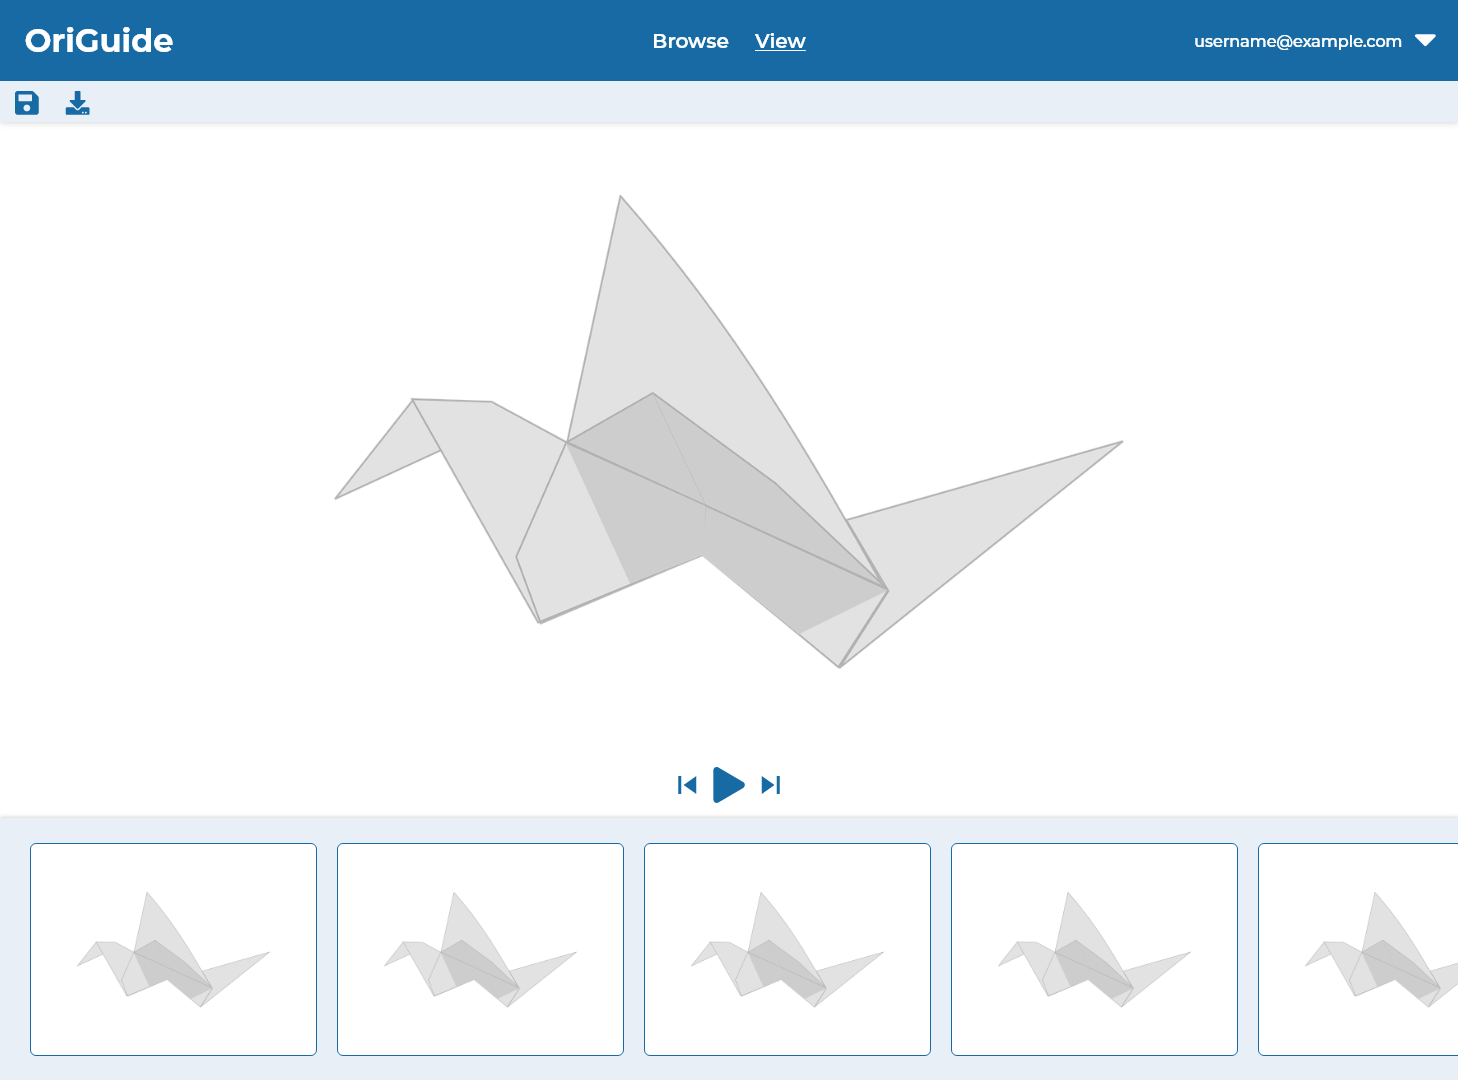
\includegraphics[width=0.8\textwidth]{assets/simulator-wireframe.png}
\end{figure}

\begin{figure}[H]
\caption{Community view}
  \centering
    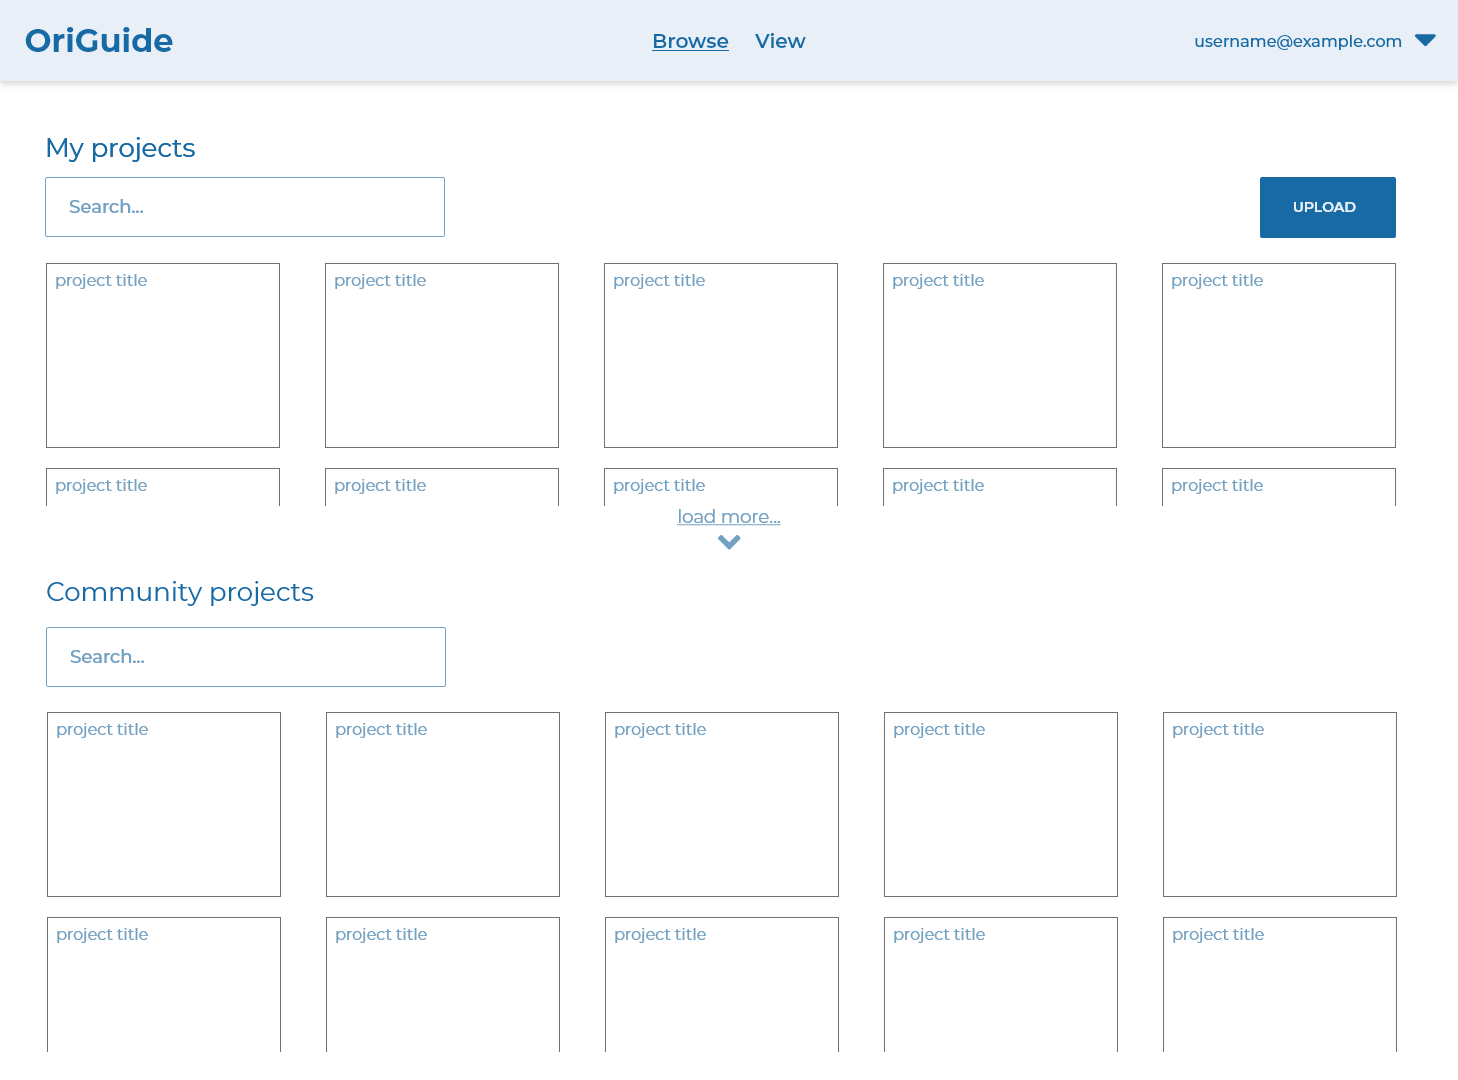
\includegraphics[width=0.8\textwidth]{assets/browser-wireframe.png}
\end{figure}
